
\documentclass{acmsiggraph}               % final
%\documentclass[review]{acmsiggraph}      % review
%\documentclass[widereview]{acmsiggraph}  % wide-spaced review
%\documentclass[preprint]{acmsiggraph}    % preprint

%% Uncomment one of the four lines above depending on where your paper is
%% in the conference process. ``review'' and ``widereview'' are for review
%% submission, ``preprint'' is for pre-publication, and ``final'' is for
%% the version to be printed.

%% These two line bring in essential packages: ``mathptmx'' for Type 1
%% typefaces, and ``graphicx'' for inclusion of EPS figures.

\usepackage{mathptmx}
\usepackage{graphicx}
\usepackage{epsfig}
\usepackage{amsmath,amscd,amssymb}
\usepackage{hyperref}

\newtheorem{theorem}{Theorem}[section]
\newtheorem{proposition}[theorem]{Proposition}
\newtheorem{definition}[theorem]{Definition}
\newtheorem{lemma}[theorem]{Lemma}
\newtheorem{corollary}[theorem]{Corollary}
\newtheorem{remark}[theorem]{Remark}


%% use this for zero \parindent and non-zero \parskip, intelligently.

\usepackage{parskip}

%% If you are submitting a paper to the annual conference, please replace
%% the value ``0'' below with your OnlineID. If you are not submitting this
%% paper to the annual conference, you may safely leave it at ``0'' -- it
%% will not be included in the output.

\onlineid{papers\_0142}

%% need to document this!

\acmformat{cameraready}

%% Paper title.

\title{Proposal: Visualizing the Loss Landscape of Neural Nets}

%% Author and Affiliation (single author).

%%\author{Roy G. Biv\thanks{e-mail: roy.g.biv@aol.com}\\Allied Widgets Research}

%% Author and Affiliation (multiple authors).

\author{Charles Ison\thanks{\small\texttt{e-mail: \{isonc|morgamat\}@eecs.oregonstate.edu}}\\ Oregon State University
\and Matthew Morgan$^{\ast}$ \\
Oregon State University}

%% Keywords that describe your work.

\keywords{rotational symmetry, field design, scalar field topology,
surfaces, topology.}

%%%%%% START OF THE PAPER %%%%%%

\begin{document}

\teaser{
	%\centerline{\epsfig{file=images/teaser.eps,angle=0,width=\textwidth}}
	$\begin{array}{@{\hspace{-0.00in}}c@{\hspace{0.05in}}c@{\hspace{0.05in}}c@{\hspace{0.05in}}c}
			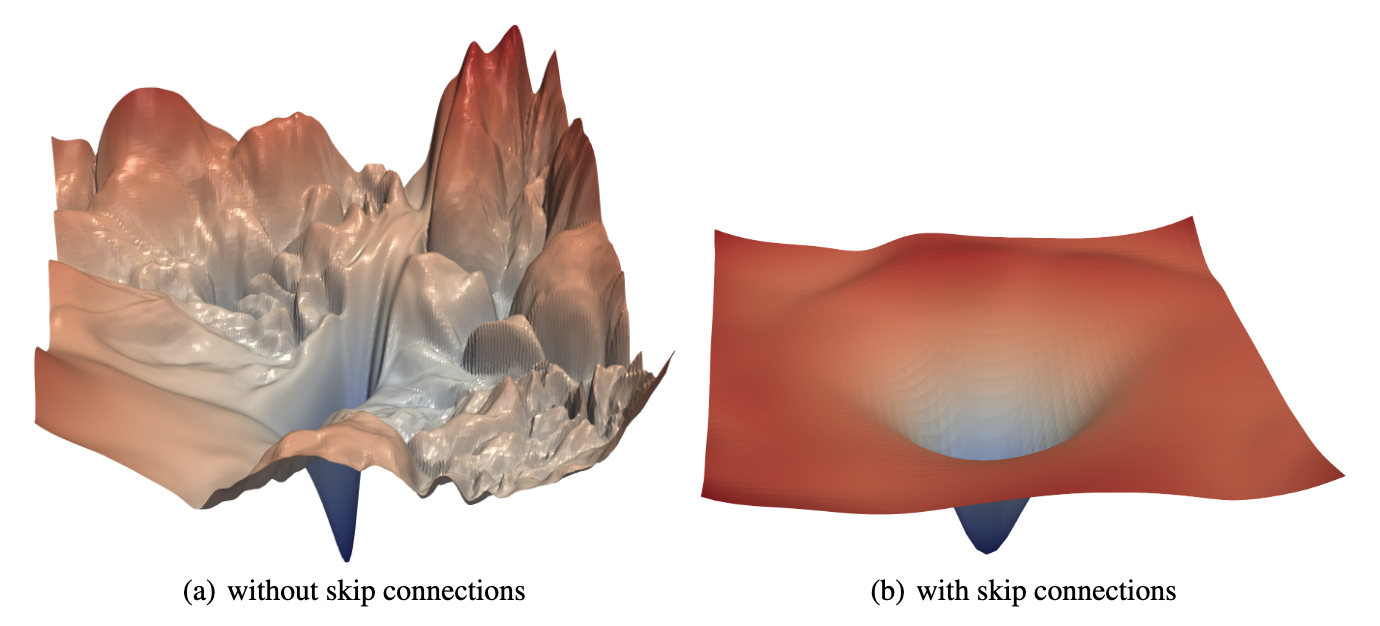
\includegraphics[width=5.50in]{/Users/mattm/repos/cs_453/sv_term_project/proposal/images/scalar-field-teaser.png}
			\\
		\end{array}$
	\caption{Example of a loss landscape visualization from the paper: (a) without skip connections, (b) with skip connections. 
		We propose to implement these visualizations as the first step of our term project, then proceeding with creating other visualizations and enhancing them. } \label{fig:teaser} }

%% The ``\maketitle'' command must be the first command after the
%% ``\begin{document}'' command. It prepares and prints the title block.

\maketitle

%% Abstract section.

\begin{abstract}

	\copyrightspace

	The abstract will be written in the final report...

\end{abstract}

%% ACM Computing Review (CR) categories.
%% See <http://www.acm.org/class/1998/> for details.
%% The ``\CRcat'' command takes four arguments.

\begin{CRcatlist}
	\CRcat{I.3.5}{Computer Graphics}{Computational Geometry and
		Object Modeling}{Geometric algorithms, languages, and systems};
\end{CRcatlist}

%% The ``\keywordlist'' command prints out the keywords.
\keywordlist


\section{Introduction}
\label{sec:intro}


%% The ``\copyrightspace'' command must be the first command after the
%% start of the first section of the body of your paper. It ensures the
%% copyright space is left at the bottom of the first column on the first
%% page of your paper.


For our term project, we propose that the paper "Visualizing the Loss Landscape of Neural Nets" (\url{https://arxiv.org/pdf/1712.09913.pdf}) be used for Option 2 (implementing a published research paper). 
In this paper, the authors create scalar field visualizations of various neural network architectures that they call “Loss Landscapes.” In these visualizations, the loss function’s results serve as the scalar value and a two dimensional reduction of the model’s weights serves the directional elements of the field. 
The specific loss functions used in the original paper are cross entropy (\url{https://pytorch.org/docs/stable/generated/torch.nn.CrossEntropyLoss.html}) and mean squared error (\url{https://pytorch.org/docs/stable/generated/torch.nn.MSELoss.html}). 
The dimensionality reduction is done using two different approaches: principal component analysis and random vector selection. 
For the later approach, two random vectors within the input space created by sampling a random Gaussian distribution. These vectors are used as the two dimensions of the scalar field input.
The resulting loss landscapes generated can then provide insights about how certain architectural decisions can improve or worsen a network's trainability.

Just like the original authors, we will have to generate our own datasets by creating test models of multiple popular neural network architectures and recording their performance across a range of weights. 
The original authors tested ResNet and VGG architectures with various permutations, which we can recreate and also potentially extend to newer architectures such as a Vision Transformer (\url{https://arxiv.org/pdf/2010.11929v2.pdf}). 
To create our loss dataset, we will also use the CIFAR-10 dataset (\url{https://www.cs.toronto.edu/~kriz/cifar.html}) as input into our testing models like the original paper. 
The models will be created in Python using PyTorch and then our results exported to PLY files which we will use to generate corresponding visualizations in OpenGL.

To evaluate the correctness of our models we will use four separate criteria. 


\begin{enumerate}
	%\itemsep 0pt
	%\parskip -1pt
	\item First, we will confirm that our results align with the original papers, which includes both quantitatively confirming our model’s performance aligns with the expected results and visually confirming our loss landscapes align with those presented in the paper. 
	\item Second, we will extract all critical points from our field, classify them using a Hessian, and confirm they match the expected values based on the scalar field visualization. 
	\item Third, the original authors visualized their model’s convergence to a local minimum during gradient descent, as seen in  Figure \ref{fig:descent_trajectory}. We will compare our local minimum with theirs to verify our accuracy.
	\item Finally, we will judge our visualization’s overall usefulness by the ability to draw meaningful insights about neural network’s architectures from the visualization. For example, the original authors were able to gain an intuition about the impact of increasing network depth and its impact on convexity. 
	Our visualizations should be of a high enough quality to convey the same information.
\end{enumerate}


\section{Previous Work}
\label{sec:previous_work}

There has been a significant amount of work in the analysis and
design of vector and tensor fields. In contrast, relatively little
is known about $N$-RoSy fields when $N \ge 3$.

	{\bf $N$-RoSy Analysis and Design:} To the best of our knowledge,
Hertzmann and Zorin~\shortcite{Hertzmann:00} are the first to
propose that hatches should follow a cross field ($4$-RoSy). They
provide a smoothing operation on $4$-RoSy fields that is based on a
non-linear optimization. Ray et al.~\shortcite{Ray:06} construct a
periodic global parameterization that facilitates quad remeshing. At
the heart of their approach is the use of $4$-RoSy fields, which
allows more natural-shaped quads to be generated near singularities.
They also develop a framework that allows the optimization to be
performed on the sines and cosines of the parameterization, which
turns a non-linear optimization into a linear one. They later
provide the analysis of singularities on $N$-RoSy's by extending the
Poincar\'e-Hopf theorem as well as describe an algorithm in which a
field with a minimal number of singularities can be constructed
based on user-specified constraints and the Euler characteristic of
the underlying surface~\cite{ray:07}.

{\bf Vector and Tensor Field Design:} There have been a number of
vector field design systems for surfaces. Most of them are generated
for a particular graphics application such as texture
synthesis~\cite{Praun:00,Turk:01,Wei:01}, fluid
simulation~\cite{Stam:03}, and vector field
visualization~\cite{vanWijk:02,vanWijk:03}. These systems do not
address topological control in the field. Systems providing
topological control include~\cite{Theisel:02,Zhang:06}. The system
of Zhang et al. has also been extended to create periodic
orbits~\cite{Chen:07} and to design tensor fields~\cite{NEURIPS2018_a41b3bb3}.
Our system is also reminiscent of the vector field design system of
Zhang et al.~\shortcite{Zhang:06} in terms of the functionality.
However, the implementation is rather different.

	{\bf Vector and Tensor Field Analysis:} There has been much work in
vector and tensor field analysis. To review all the work is beyond
the scope of this paper. Here we refer to the most relevant work.
Helman and Hesselink~\shortcite{Helman:91} propose vector field
visualization techniques based on topological analysis. Delmarcelle
and Hesselink provide analysis of second-order symmetric tensor
fields~\shortcite{NEURIPS2018_a41b3bb3}.

%Cabral and Leedom present a texture-based visualization for vector
%fields, which they termed {\em LIC} (Line-integral
%convolution)~\cite{Cabral:93}. This technique is of high quality.
%Later, van Wijk~\shortcite{vanWijk:02,vanWijk:03} provides an
%image-based flow visualization technique (IBFV) that is of similar
%quality but much faster due to the use of graphics hardware. Zhang
%et al.~\shortcite{Zhang:07} extend IBFV to symmetric second-order
%tensor fields.

\section{Vector-Based Representation}
\label{sec:representation}

TODO...



\begin{figure}[t]
	\begin{center}
		$\begin{array}{@{\hspace{-0.00in}}c@{\hspace{0.05in}}c}
				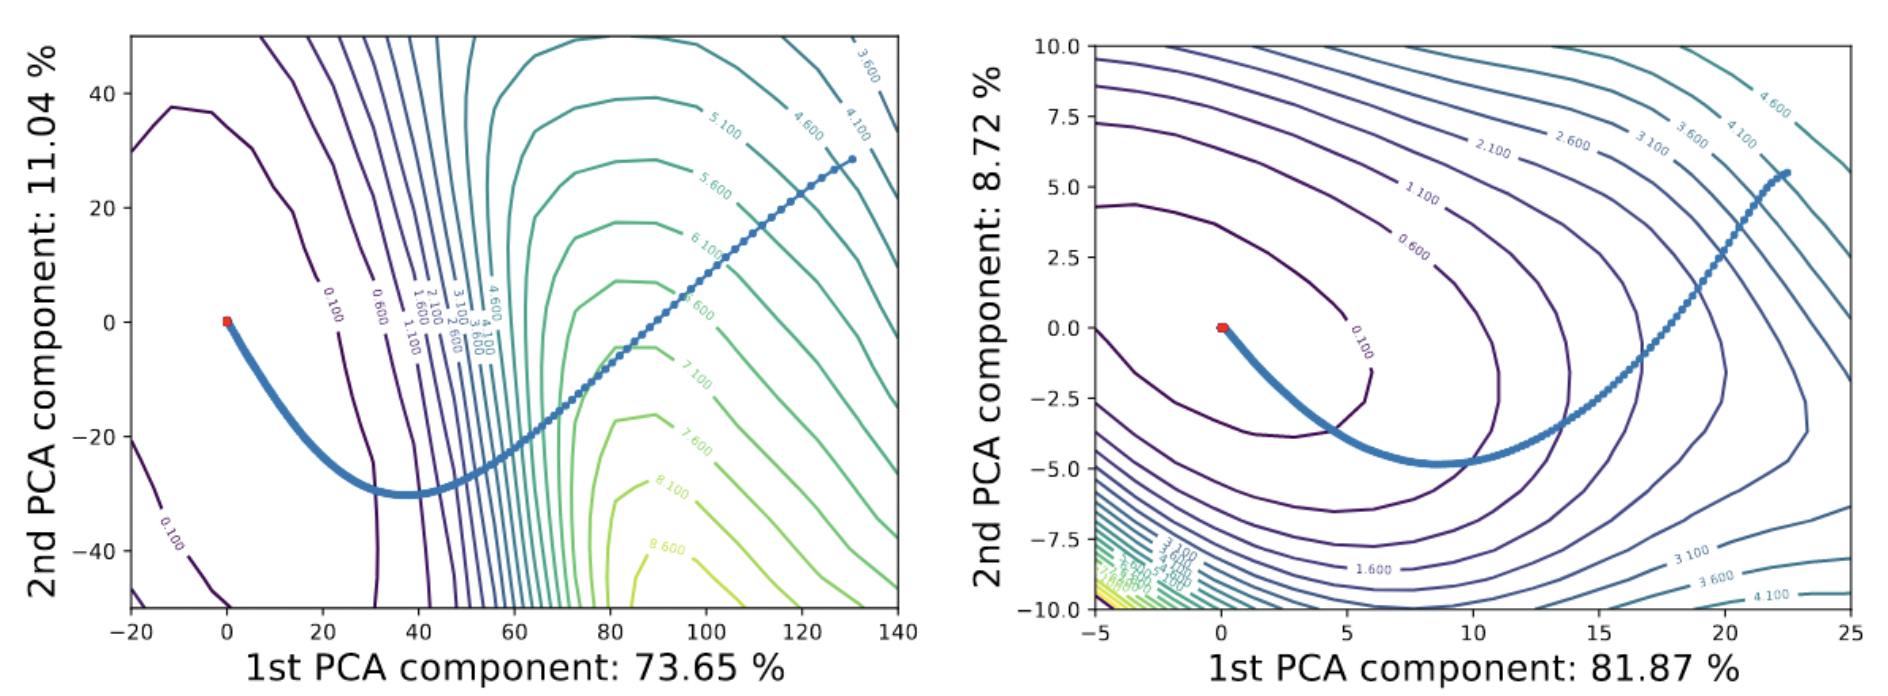
\includegraphics[height=1.07in]{images/traj-plot-SGD.png}
				\\
			\end{array}$
	\end{center}
	\caption{ Plots from the original authors visualizing the model's convergence to a local minimum during gradient descent. } \label{fig:descent_trajectory}
\end{figure}

\section{Topological Analysis of $N$-RoSy Fields}
\label{sec:analysis}

In this section, TODO...

\section{Design of $N$-RoSy Fields}
\label{sec:design}

In this section, TODO\dots



\section{Applications}
\label{sec:application}

We have applied our design system to pen-and-ink sketching and
quad-dominant remeshing.


\subsection{Example Subsection}
\label{sec:pen_and_ink}

Subsection, TODO\dots



\section{Conclusion}
\label{sec:conclusion}

The conclusion will be written in the final report.


\section*{Appendix}
\label{sec:higher_tensors}

To be determined.

\section*{Acknowledgements}

To be determined.


\bibliographystyle{acmsiggraph}
\nocite{*}
\bibliography{nn_loss}
\end{document}
